\chapter{Análisis Estructural}

\section{Análisis Preliminar}
Los difractogramas obtenidos fueron analizados con el programa
X'Pert$^{\textregistered}$ High Score, en donde, se realizó un análisis preliminar
para determinar la correcta sinterización del granate mediante la comparación
con los registros de la base de datos PDF 2 (2004). A partir de los resultados
obtenidos se determinó que para el material sin sustitución de aluminio (con
x=0.0 \ce{Al5Lu3O12}) hay presencia de la fase cristalina correspondiente al
granate de lutecio aluminio-LUAG (\ce{Al5Lu3O12}) como fase mayoritaria,
identificada con el código de fichero 01-073-1368, que tiene como
características: estructura cúbica y grupo espacial Ia-3d (230). Además, se
encontró presencia de óxido de lutecio (\ce{Lu2O3}) con código 01-086-2475 como
fase minoritaria, de estructura cristalina cubica, grupo espacial Ia-3d (206).
El \ref{AnexoA}-1 muestra el difractograma del \ce{Al5Lu3O12}, en el cual se logran
identificar las fases presentes en el material. Este análisis preliminar se
realizó para todos los difractogramas de DRX obtenidos de cada material del sistema
\ce{Lu3Al_{5-X}Fe_{x}O12}:\ce{Ce^{3+}}, con la finalidad de confirmar la
presencia del granate como fase mayoritaria, las imágenes de los resultados se
presentan en el Anexo \ref{AnexoA}.\\

Los difractogramas obtenidos de cada uno de los materiales del sistema
\ce{Lu3Al_{5-X}Fe_{x}O12}:\ce{Ce^{3+}} (con 0.0 $\leq$ x $<$ 4.5) se agruparon
y se presentan en la Figura \ref{fig:patDRX}. Donde, se pudo determinar
mediante análisis gráfico que se tiene un ligero desplazamiento de las señales
de difracción hacia ángulos inferiores de 2 $\theta$ (ver parte derecha de la
Figura \ref{fig:patDRX}), lo que se relaciona con el aumento de la
concentración de \ce{Fe^{3+}}. Esta variación se atribuye al radio iónico del
\ce{Fe^{3+}} (r = 6.75 \r{A}) que es mayor al radio del \ce{Al^{3+}} (r = 5.85
\r{A}) \cite{Deng2013}. También se observaron señales del difractograma que indican la
presencia de fases cristalinas secundarias para valores de x menores o iguales
a 2.0 (x $\leq$ 2.0) marcadas en la  con (*).

\begin{figure}[h]
    \centering%

    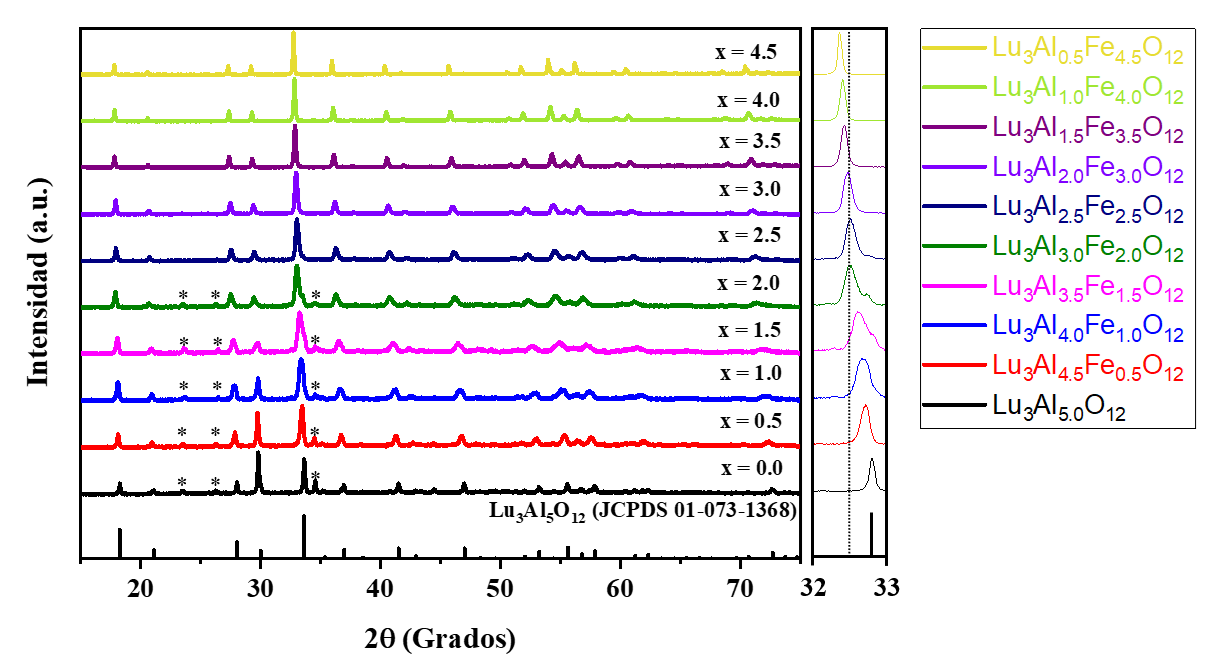
\includegraphics[width=\textwidth]{Kap3/PatronesDRX.png}%
    \caption{Difractogramas DRX de las muestras
    \ce{Lu3Al_{5-X}Fe_{x}O12}:\ce{Ce^{3+}} con 0.0 $\leq$ x $<$4.5; (*)
    Indica las
    señales de difracción asociados a las fases cristalinas secundarias.
    Panel
    derecho:  difractogramas ampliados en el rango de 2$\theta$ 32–33$^o$.}
    \label{fig:patDRX}
\end{figure}

En la Figura \ref{fig:DRXamp} se presenta la región ampliada de 32 a 34 grados
de la señal principal de los difractogramas del sistema
\ce{Lu3Al_{5-X}Fe_{x}O12}:\ce{Ce^{3+}}, en donde, se aprecia mejor la similitud
de cada una de las señales obtenidas y la tendencia del desplazamiento hacia
valores menores de 2$\theta$, también se indica en la figura la relación de los
difractogramas con el aumento de la concentración de \ce{Fe^{3+}} y la
disminución de \ce{Al^{3+}}.

\begin{figure}[h]
    \centering%

    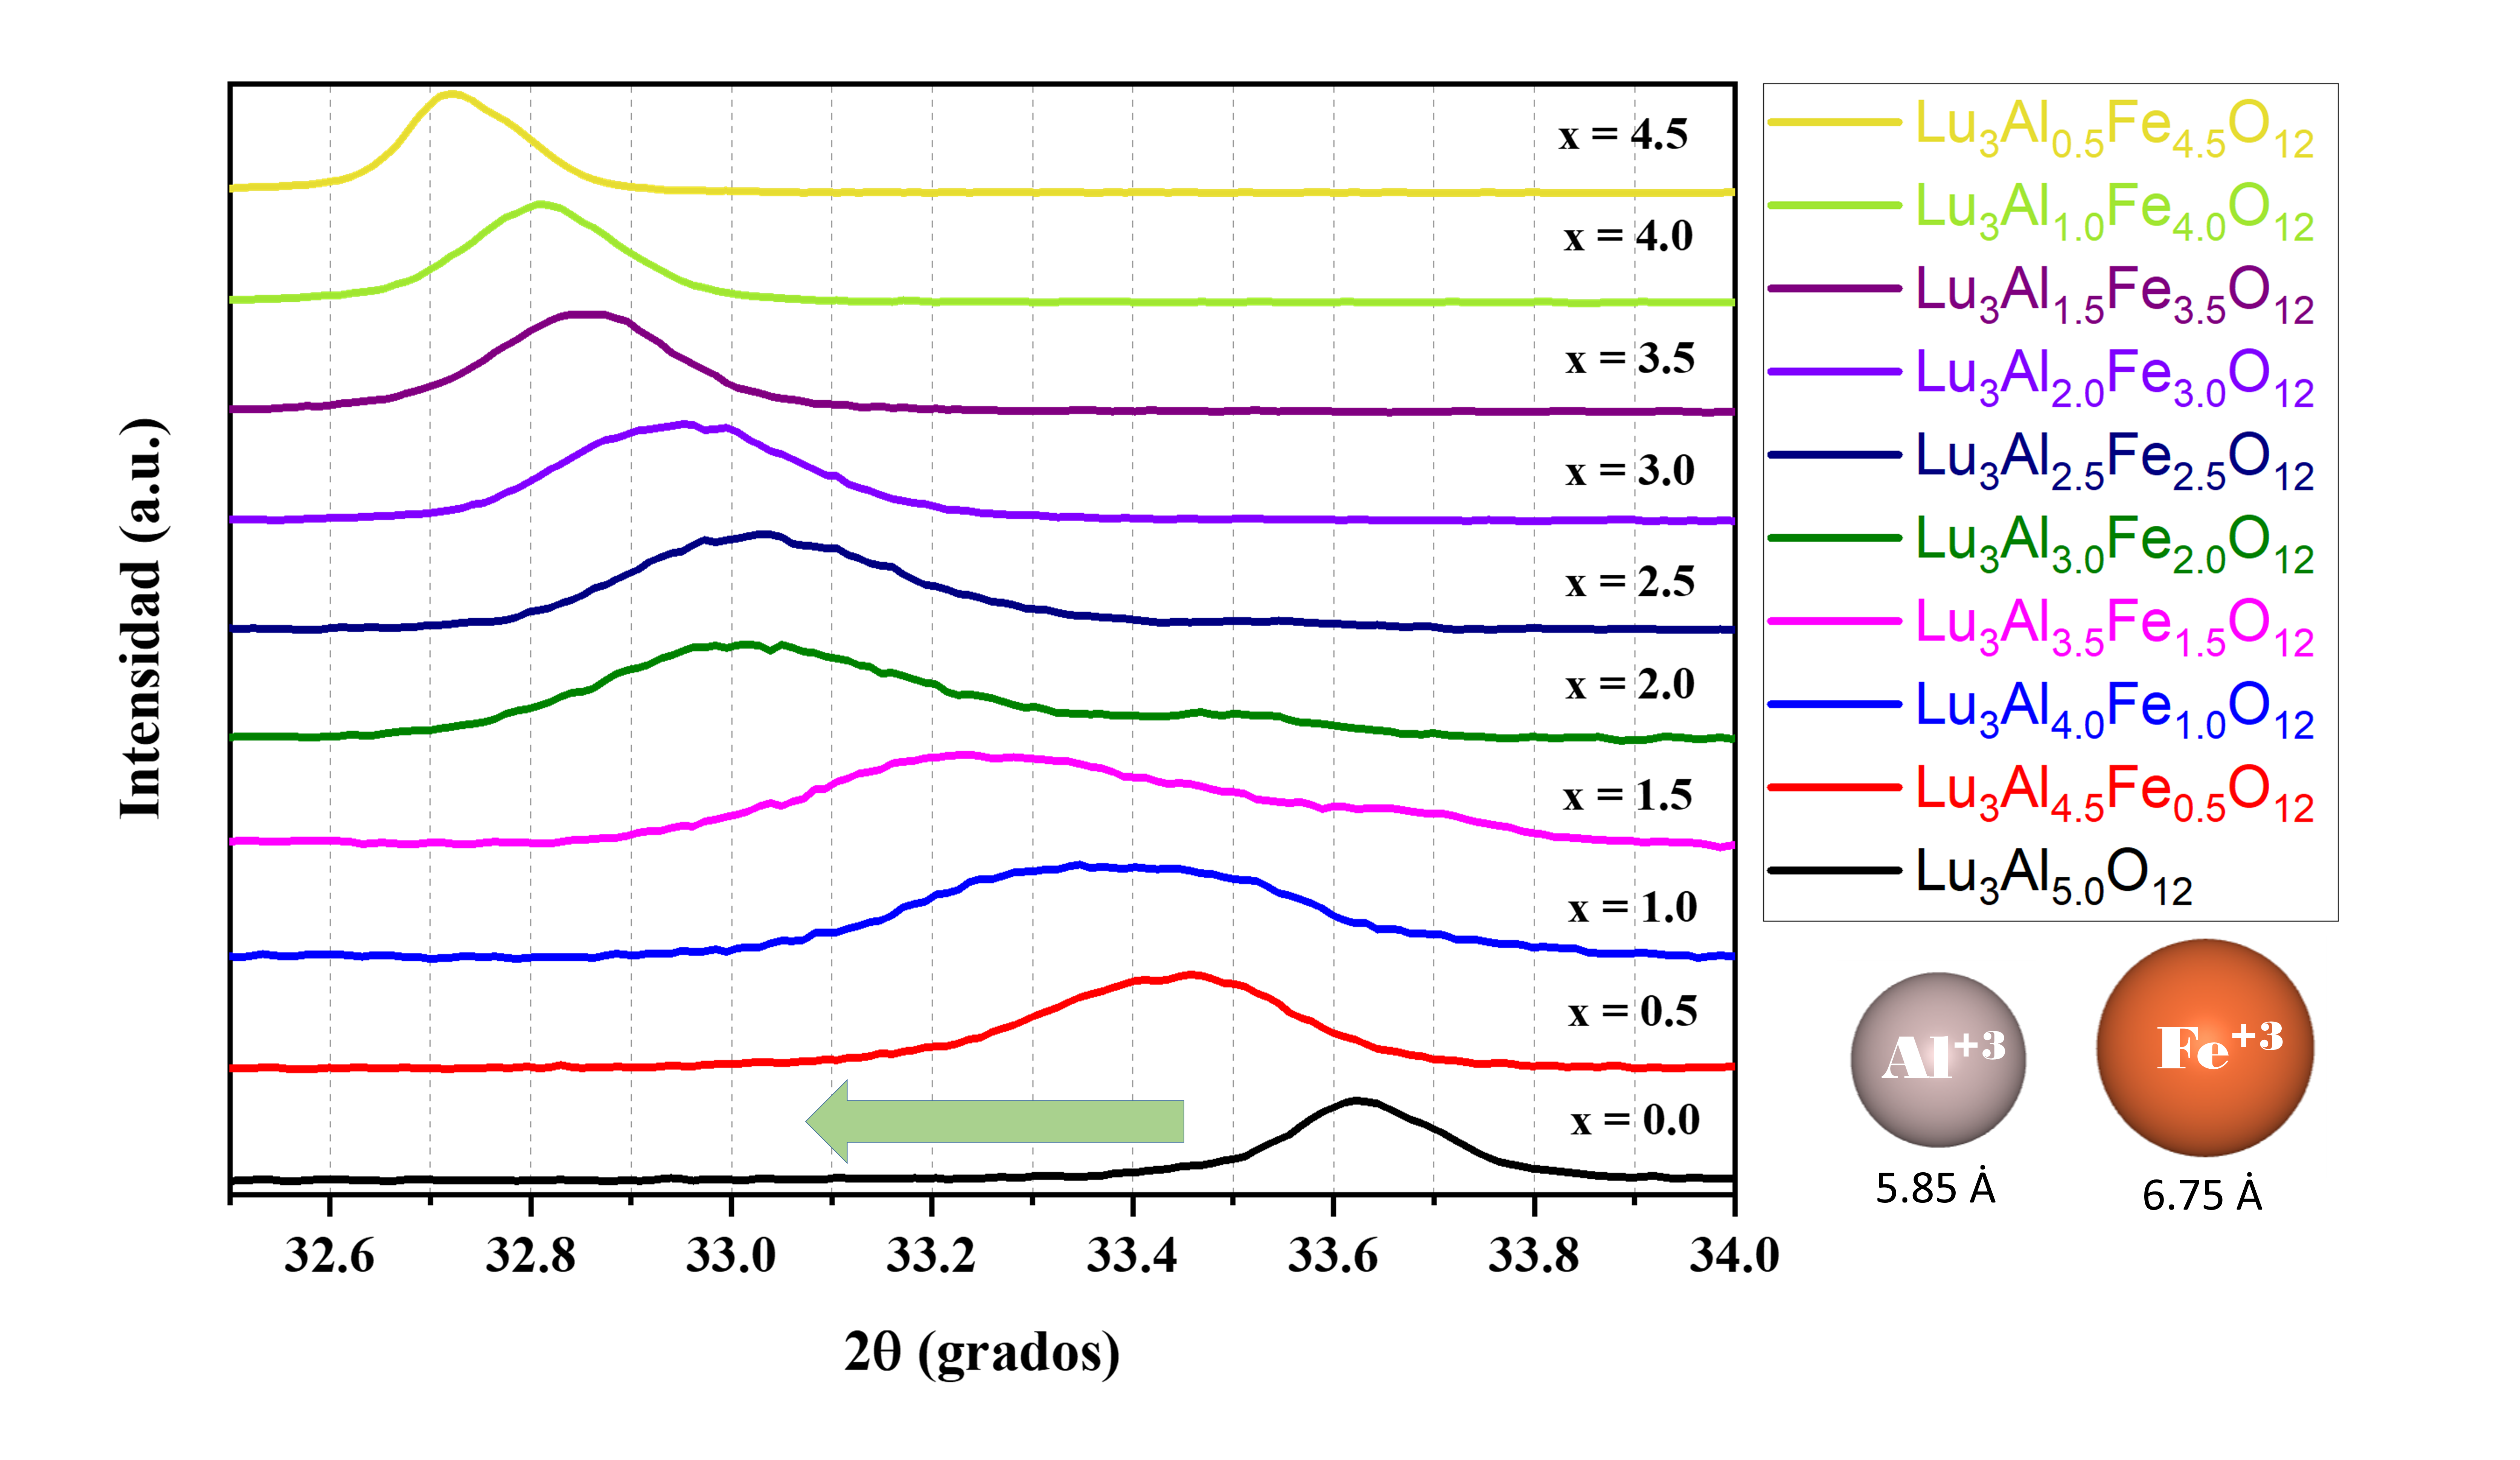
\includegraphics[width=\textwidth]{Kap3/DRXampliado.png}%
    \caption{Región ampliada de la señal principal del sistema de los
    difractogramas DRX de las muestras \ce{Lu3Al_{5-X}Fe_{x}O12}:\ce{Ce^{3+}} en el rango
    de
    2$\theta$ 32–33$^o$} \label{fig:DRXamp}
\end{figure}

\section{Refinamiento Rietveld}

El análisis preliminar realizado con el programa X’Pert\textregistered High
Score permitió
identificar las fases cristalinas presentes en cada material, y sirvió como
punto de partida para proceder con un análisis más detallado mediante el método
de refinamiento Rietveld, apoyado en el uso del software PCW y GSAS, con la
finalidad de determinar los parámetros estructurales y la composición de todas
las muestras producidas para el sistema \ce{Lu3Al_{5-X}Fe_{x}O12}:\ce{Ce^{3+}}
(x= 0.0, 0.5, 1.0, 1.5, 2.0, 2.5, 3.0, 3.5 y 4.5). En la Figura \ref{fig:refi}
se pueden observar los difractogramas refinados para x=0.0 y x=4.5 los demás se
presentan en el Anexo \ref{AnexoB}. Los símbolos (x) representan los difractogramas 
experimentales, la línea roja el difractograma refinado, las barras verticales ($\mid$)
representan las posiciones de Bragg de cada fase identificada, en verde se
muestra el ruido, en azul la diferencia entre el difractograma experimental y el
teórico.\\

\begin{figure}[h]
    \centering%

    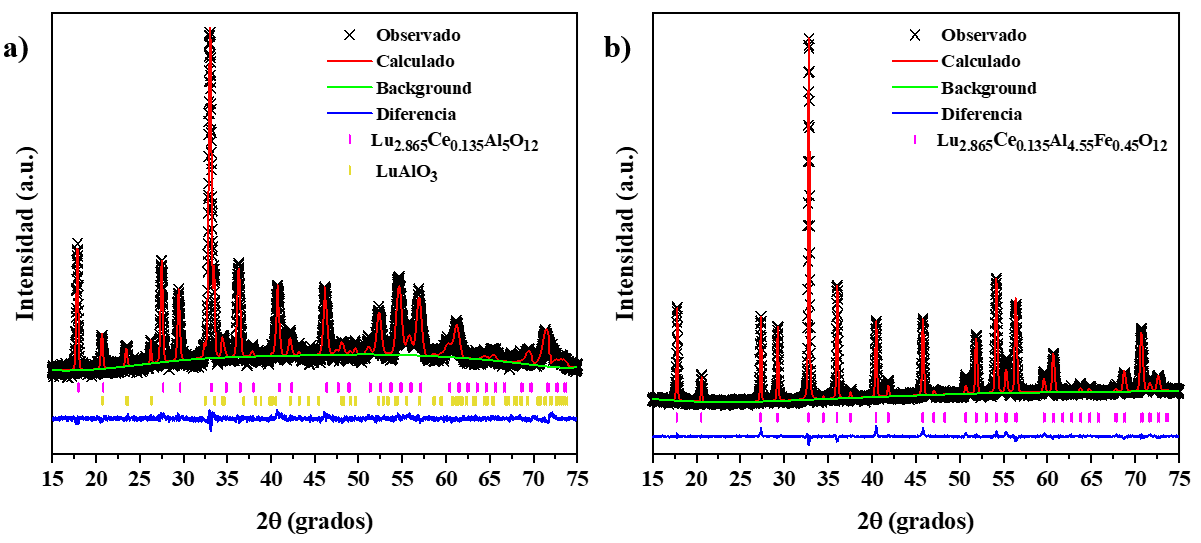
\includegraphics[width=\textwidth]{Kap3/Refinamiento.png}%
    \caption{Difractogramas refinados de DRX para muestras del sistema
    \ce{Lu3Al_{5-X}Fe_{x}O12}, con a) x=0.0, b) x=4.5} \label{fig:refi}
\end{figure}

Los datos estructurales y los factores residuales de cada una de las muestras
se pueden ver en la Tabla 2. Datos estructurales y factores residuales de las
muestras de \ce{Lu3Al_{5-X}Fe_{x}O12}:\ce{Ce^{3+}}, donde se determinó la
presencia como fase cristalina principal el granate \ce{Lu3Al5O12} (JCPDS
01-073-1368) con estructura cubica y grupo espacial l3d (230). Para
concentraciones bajas de \ce{Fe^{3+}} (0.0 $\leq$ x $\leq$ 4.5) se identificó
como
fase secundaria el \ce{LuAlO3} (JCPDS 00-024-0690). Sin embargo, se obtuvieron
materiales de fase única partir de valores de x mayores o iguales a 2.5 (x
$\geq$ 2.5), lo que se le atribuye a la menor temperatura de fusión del
precursor de \ce{Fe^{3+}} comparada con la del \ce{Al^{3+}}, la cual favoreció
la difusión iónica y la formación la estructura del granate.\\

En la Figura \ref{fig:para} a) se presenta la relación entre el parámetro de
red de la
celda unidad y el aumento de la concentración \ce{Fe^{3+}}, donde se tiene una
tendencia lineal hacia la expansión de la celda unidad, que se puede relacionar
con el desplazamiento de las señales de DRX y también confirma la sustitución
de \ce{Fe^{3+}} por \ce{Al^{3+}} en la estructura del granate, al relacionarse
con la Ley de Vegard, que indica que el parámetro de red de la estructura
cristalina
resultante es una media ponderada de los constituyentes \cite{Kempter1966,King1921}. En la Figura
\ref{fig:para}
b) podemos observar representación en tres dimensiones (3D) de la celda unidad
siguiendo
los datos obtenidos del refinamiento para el sistema granate
\ce{Lu3Al_{5-X}Fe_{x}O12}:\ce{Ce^{3+}}, donde, los átomos de Lu y Ce ocupan los
sitios 24(c) formando un dodecaedro, los átomos de Al y Fe ocupan los sitios
24(d) formando un tetraedro, y los sitios 16(a) formando un octaedro.\\

\begin{figure}[h]
    \centering%

    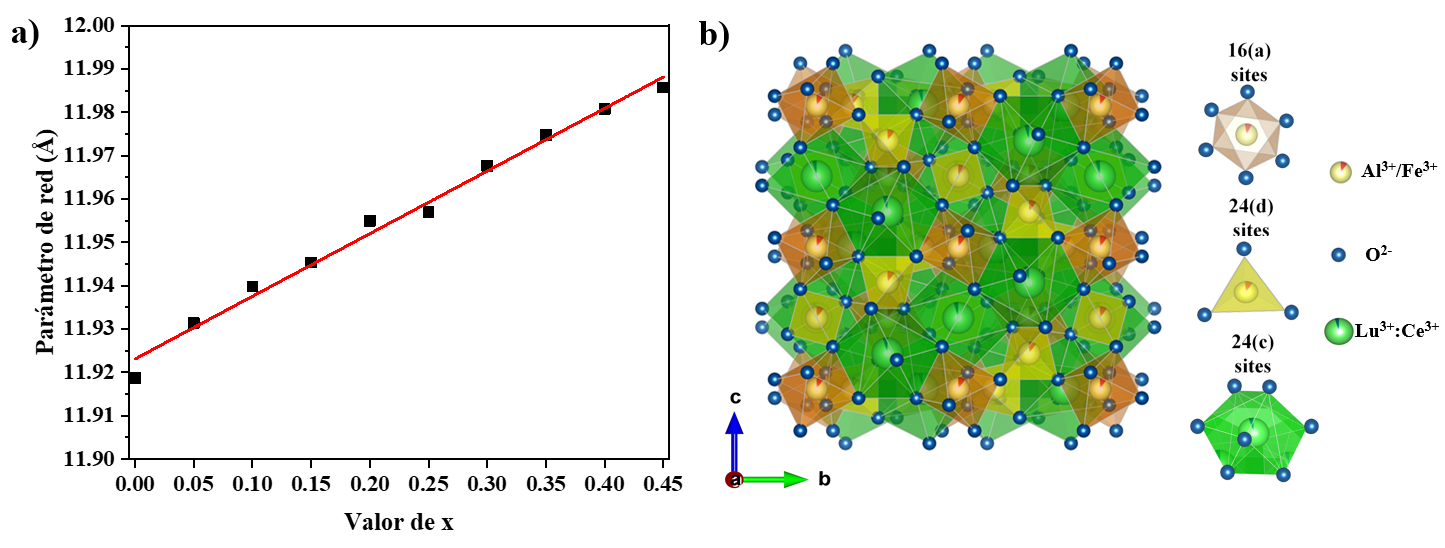
\includegraphics[width=\textwidth]{Kap3/ParametroRed.png}%
    \caption{Parámetro de red a como función de la concentración de
    \ce{Fe^{3+}}
    (valor de x) y una vista en 3D de la celda unitaria del sistema granate
    \ce{Lu3Al_{5-X}Fe_{x}O12}:\ce{Ce^{3+}}}
    \label{fig:para}
\end{figure}

\section{Espectroscopia del Infrarrojo Cercano}

Se registraron espectros de absorción en la región de infrarrojos cercanos
(NIR) para verificar la modificación de las bandas electrónicas y vibratorias,
generadas por la inserción \ce{Fe^{3+}} en la estructura del granate. En La
Figura \ref{fig:nir} se presentan los espectros NIR para las muestras del
sistema
\ce{Lu3Al_{5-X}Fe_{x}O12}:\ce{Ce^{3+}} (x = 0.0 y 4.5).\\

\begin{figure}[h]
    \centering%

    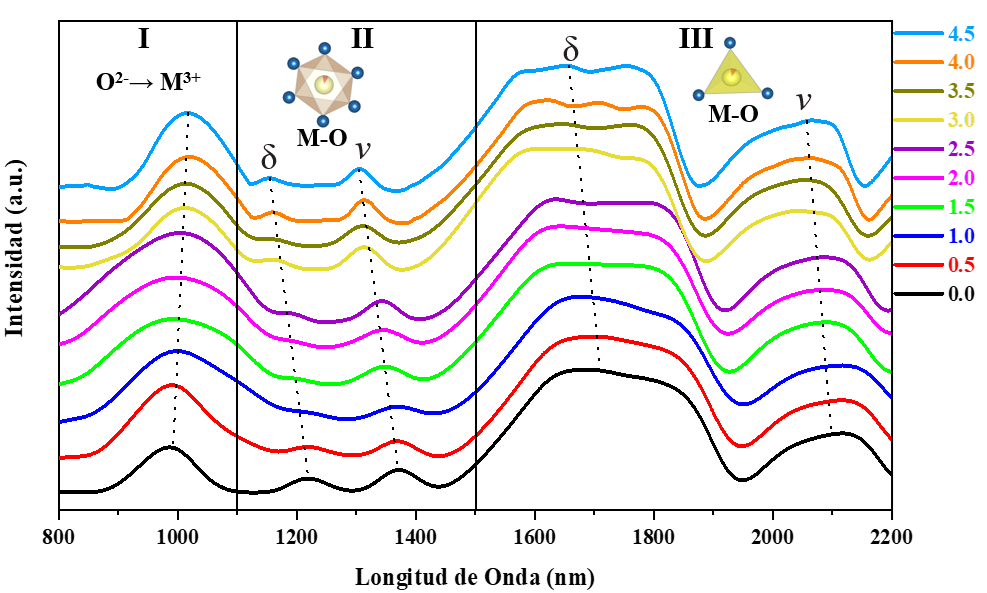
\includegraphics[width=\textwidth]{Kap3/NIR.png}%
    \caption{Espectros de absorción en la región NIR para las muestras
    \ce{Lu3Al_{5-X}Fe_{x}O12}:\ce{Ce^{3+}} (0.0 $\leq$ x $\leq$ 4.5)}
    \label{fig:nir}
\end{figure}

Los espectros se pueden separar en tres regiones principales, a las que se
atribuyen: absorción electrónica debido a la transferencia de carga
oxígeno-metal (I), y absorciones vibratorias atribuidas al estiramiento ($\upsilon$ ) y
flexión ($\sigma$) de la unión metal-oxígeno en configuraciones octaedro (II) y
tetraedro (III). Las bandas asociadas a la transferencia de carga oxígeno-metal
se encuentran en el rango espectral 800-1100 nm \cite{Rossman2019}. Al aumentar la concentración
\ce{Fe^{3+}}, la banda exhibió un desplazamiento hacia longitudes de onda más largas
(disminución de la energía), esto se atribuye a las variaciones en los
poliedros locales y la mezcla de estados excitados \cite{Krambrock2013}. Los cationes trivalentes
exhiben un mayor radio iónico efectivo cuando
están en configuración octaédrica, y existe una mayor repulsión electrostática
de los seis átomos de oxígeno que los rodean. Entonces, las bandas atribuidas a
la absorción vibracional de la configuración octaédrica se ubican en longitudes
de onda más cortas que las de la configuración tetraédrica \cite{Rossman2019}. La longitud de
onda de las absorciones vibratorias es proporcional al poder de polarización
del catión en una configuración octaédrica o tetraédrica. El catión \ce{Fe^{3+}} tiene
un poder de polarización menor (4.76) que el \ce{Al^{3+}} (5.66) \cite{Bishop2019}, por lo tanto, una
mayor concentración de \ce{Fe^{3+}} en los granates condujo a una disminución
progresiva en la longitud de onda de las absorciones vibratorias.